\begin{figure}[htbp]
\centering
\begin{tikzpicture}[schema base]
\node[schema titolo] at (0,0.3) {Conteggio visibile e conteggio generato};
\node[schema nota,anchor=west] at (0,-0.35) {Asset digitale originale -- pagina 225, chiamata 0004};
\node[anchor=north west,inner sep=0] at (0.3,-0.9)
  {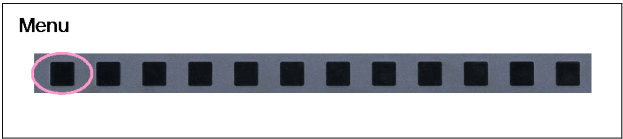
\includegraphics[width=14.4cm]{figure/asset/v4/docling-image-0225-0010.png}};
\foreach \numero/\pixel in {1/62,2/108,3/154,4/200,5/246,6/292,7/338,8/384,9/430,10/476,11/522,12/568} {
  \draw[schema icona,draw=schemaBlu!70,line width=0.5pt]
    ({0.3+14.4*\pixel/623},-4.6) -- ({0.3+14.4*\pixel/623},{-0.9-14.4*92/623});
  \node[font=\schemafont\footnotesize,text=schemaBlu] at ({0.3+14.4*\pixel/623},-4.95) {\numero};
}
\node[schema nota,text width=14cm] at (7.5,-5.55)
  {Numerazione editoriale aggiunta per rendere controllabile il conteggio: 12 pulsanti.};
\node[schema blocco,text width=6.2cm,minimum height=2cm] at (3.5,-7.35)
  {\textbf{Che cosa afferma la caption}\\[4pt]
  \enquote{10 pulsanti quadrati neri}\\[4pt]
  Il primo è descritto correttamente\\come cerchiato in rosa.};
\node[schema esterno,text width=6.2cm,minimum height=2cm] at (11.5,-7.35)
  {\textbf{Che cosa attestano i controlli}\\[4pt]
  Stato: \texttt{enriched}\\Inclusione prevista: attiva\\Formato accettato, conteggio non verificato};
\end{tikzpicture}
\caption{La caption di \texttt{docling-image-0225-0010} conta dieci pulsanti, ma nell'immagine sono dodici: il controllo di formato non rileva l'errore. Numeri e linee sono aggiunti per il confronto; il cerchio rosa è nell'originale.}
\label{fig:errore-caption-menu}
\end{figure}